\section{Pattern Description}

\begin{frame}[fragile]{History of \patternname}
	\begin{columns}[T,onlytextwidth]
		\begin{column}{0.6\textwidth}
			\begin{itemize}
				\item Introduction by Bjarne Stroustrup in the early 1990s as part of C++ design
				      \begin{itemize}
					      \item Programming Idiom: \textit{Common, conventional way of writing code to solve a recurring problem}
				      \end{itemize}
				\item Its purpose is to \textbf{bind resource management to object lifetime}
				      \begin{itemize}
					      \item Resources (memory, files, locks) are \textbf{acquired in Constructors}
					      \item Resources are guaranteed to be \textbf{automatically released in Destructors} (Deterministic)
				      \end{itemize}
				\item Safer code at essentially zero runtime overhead
				      \begin{itemize}
					      \item Memory-Safety
					      \item Exception-Safety
				      \end{itemize}
			\end{itemize}
		\end{column}
		\begin{column}{0.4\textwidth}
			\begin{figure}
				\centering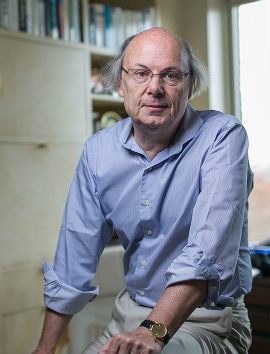
\includegraphics[height=0.5\textheight]{res/Bjarne2018.jpg}
				\caption{Bjarne Stroustrup \newline \tiny \fullcite{stroustrup_image}}
			\end{figure}
		\end{column}
	\end{columns}
	\blfootnote{\cite{cppreference_raii} \cite{isocpp_coreguidelines} \cite{Stroustrup2018-ic} \cite{Will2020-og} \cite{Meyers2014-ot}}
\end{frame}



\begin{frame}[fragile]{\patternname\ (i)}
	\begin{columns}[T,onlytextwidth]
		\begin{column}{0.6\textwidth}
			\begin{itemize}
				\item Idea:
				      \begin{itemize}
					      \item No manual \mintinline{cpp}|new|
					      \item No manual \mintinline{cpp}|delete|/\mintinline{cpp}|delete[]|
				      \end{itemize}
				\item Constructor: Initializes and Acquires Resources
				\item \textbf{Destructor}: Releases all Acquired Resources
				      \begin{itemize}
					      \item Automatically:
					            \begin{itemize}
						            \item Out of scope
						            \item Exception is thrown
					            \end{itemize}
					      \item Guaranteed by the programming language
				      \end{itemize}
			\end{itemize}
		\end{column}
		\begin{column}{0.4\textwidth}
			\begin{figure}
				\centering
				\begin{minted}{cpp}
int main() {
    int* arr = new int[10];
    // ...
    delete[] arr; // manual!
} // not exception safe!
                \end{minted}
				\rule{\linewidth}{0.5mm}
				\begin{minted}{cpp}
#include <vector>
int main() {
    std::vector<int> arr(10);
    // ...
} // automatic release
                \end{minted}
				\caption{Example: RAII vs Manual Memory Management, Array with 10 Integers on the Heap}
			\end{figure}
		\end{column}
	\end{columns}
\end{frame}

\begin{frame}[fragile]{\patternname\ (ii)}
	\begin{figure}
		\centering
		\begin{minted}{cpp}
class MyClass {
	int* m_arr;
public:
	MyClass() { // Constructor: Create Object (explicit)
		m_arr = new int[10];
	}
	~MyClass() { // Destructor: Delete Object (automatically)
		delete[] m_arr;
	}
};
int main() {
	MyClass obj; // Constructor
} // Destructor automatically runs at the end of scope
  // Even when an exception is thrown!
	    \end{minted}
		\caption{Example: RAII implementation}
	\end{figure}
\end{frame}

% TODO References!
